\documentclass{article}

% if you need to pass options to natbib, use, e.g.:
%     \PassOptionsToPackage{numbers, compress}{natbib}
% before loading neurips_2021

% ready for submission
\usepackage[preprint]{neurips_2021}

% to compile a preprint version, e.g., for submission to arXiv, add add the
% [preprint] option:
%     \usepackage[preprint]{neurips_2021}

% to compile a camera-ready version, add the [final] option, e.g.:
%     \usepackage[final]{neurips_2021}

% to avoid loading the natbib package, add option nonatbib:
%    \usepackage[nonatbib]{neurips_2021}

\usepackage[utf8]{inputenc} % allow utf-8 input
\usepackage[T1]{fontenc}    % use 8-bit T1 fonts
\usepackage[colorlinks=true]{hyperref}       % hyperlinks
\usepackage{url}            % simple URL typesetting
\usepackage{booktabs}       % professional-quality tables
\usepackage{amsfonts}       % blackboard math symbols
\usepackage{nicefrac}       % compact symbols for 1/2, etc.
\usepackage{microtype}      % microtypography
\usepackage{xcolor}         % colors
\usepackage{graphicx}

\title{Analyzing the Enron mails}

% The \author macro works with any number of authors. There are two commands
% used to separate the names and addresses of multiple authors: \And and \AND.
%
% Using \And between authors leaves it to LaTeX to determine where to break the
% lines. Using \AND forces a line break at that point. So, if LaTeX puts 3 of 4
% authors names on the first line, and the last on the second line, try using
% \AND instead of \And before the third author name.

\author{%
  Peter Heringer\\
  Matrikelnummer 6109174 \\
  \texttt{peter.heringer@student.uni-tuebingen.de} \\
  \And
  Felix Seidel\\
  Matrikelnummer 5969276 \\
  \texttt{felix.seidel@student.uni-tuebingen.de} \\
}

\begin{document}

\maketitle

\begin{abstract}
  The Enron mail corpus provides real world corporate mail communication data. 
  The corpus contains mails by Enron personell during the phase in which Enron 
  declarerd bankrupcy. We extract the core working hours of the Enron personell 
  from this dataset. The dataset indicates that Enron performed a migration 
  of their mail systems shortly before the scandal became public, which
  introduces an intersting shift in the mails' time information. However, we
  show that there is no significant change in core working hours over time.
\end{abstract}

\section{Introduction}
TODO: Introduce Enron mail corpus, briefly summarize where the data comes from
and how it was prepared BEFORE we accessed it

\section{Related work}
TODO: Briefly discuss other reports of the mail data.

\section{Analyzing the time data}
TODO: Describe our Hypothesis. Describe how we extracted the Date information, 
how we removed duplicates and show plot of the dates over time.

\begin{center}
  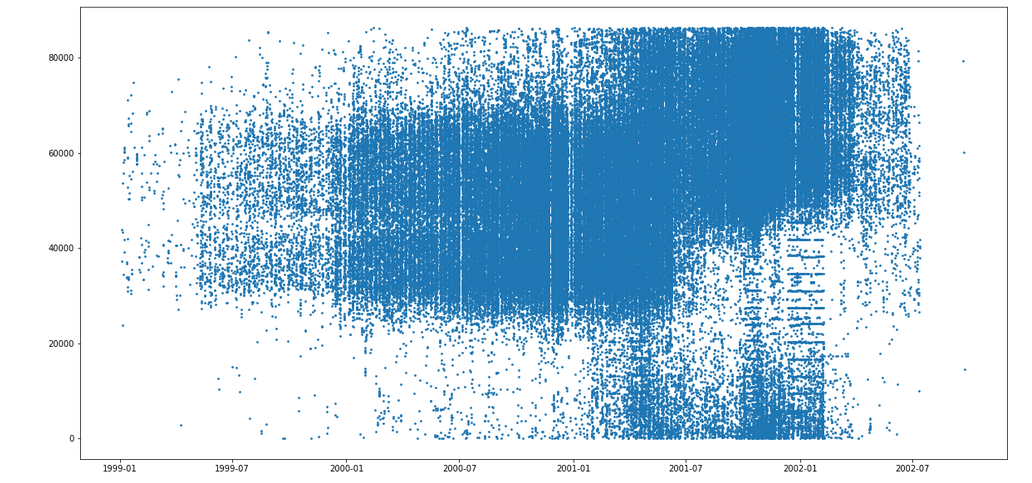
\includegraphics[width=0.7\linewidth]{tmp/plot_all_mail.png}
\end{center}

Describe the shift that appears in summer 2001
and how we connected that shift to some mail migration. To this end, plot the
mail communication of jeff.dasovich@enron.com over time with all mail data (ie.
the data where only the naive duplicate detection was performed), with the mail
data without duplicates and with the mail data extracted from just the
"sent"-folders.

\begin{center}
  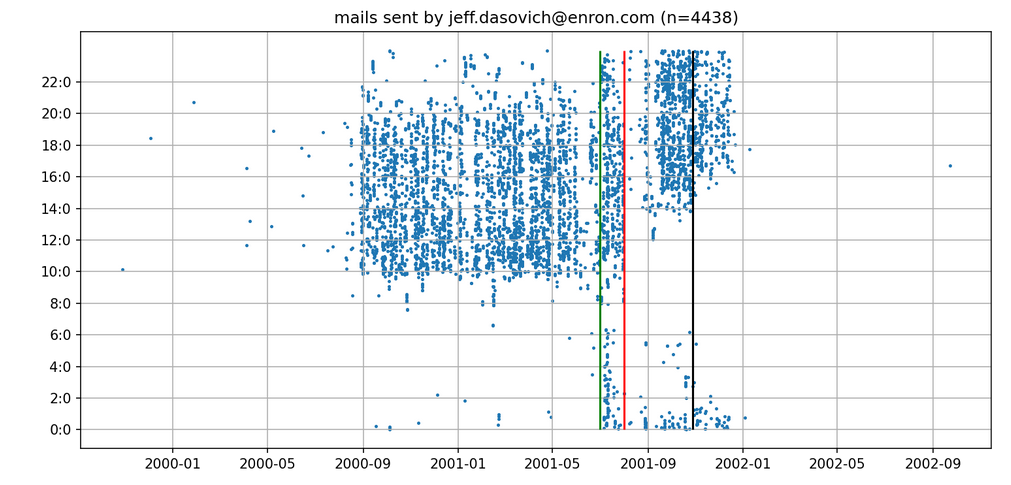
\includegraphics[width=0.7\linewidth]{tmp/plot_jeff_all.png}
\end{center}
\begin{center}
  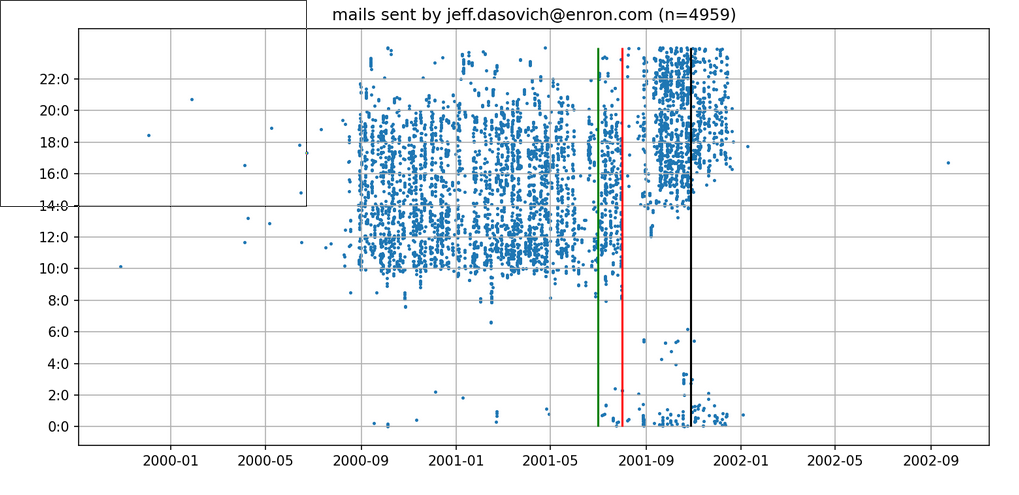
\includegraphics[width=0.7\linewidth]{tmp/plot_jeff_stripped.png}
\end{center}

Describe that this is also visible when making box plots for each month.
\begin{center}
  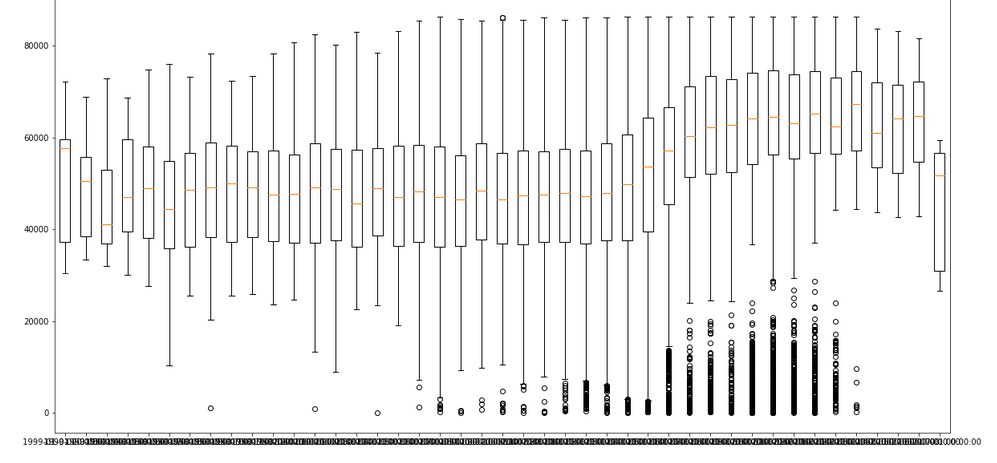
\includegraphics[width=0.7\linewidth]{tmp/boxplot_all.png}
\end{center}

Describe how we calculated the average core working hours for each month based
on that plot. Show how we tested our initial Hypothesis given that data.

\section{Discussion}
Discuss the assumptions that we've made, ie. why we can use the 25/75 quantile,
why we think we can ignore the shift in the mail data, why the assumption of
core working hours is justified.

\section{References}

\end{document}
